\documentclass[openany]{book}
\usepackage{lmodern}
\usepackage{amssymb,amsmath}
\usepackage{ifxetex,ifluatex}
\usepackage{fixltx2e} % provides \textsubscript
\ifnum 0\ifxetex 1\fi\ifluatex 1\fi=0 % if pdftex
  \usepackage[T1]{fontenc}
  \usepackage[utf8]{inputenc}
\else % if luatex or xelatex
  \ifxetex
    \usepackage{mathspec}
  \else
    \usepackage{fontspec}
  \fi
  \defaultfontfeatures{Ligatures=TeX,Scale=MatchLowercase}
\fi
% use upquote if available, for straight quotes in verbatim environments
\IfFileExists{upquote.sty}{\usepackage{upquote}}{}
% use microtype if available
\IfFileExists{microtype.sty}{%
\usepackage{microtype}
\UseMicrotypeSet[protrusion]{basicmath} % disable protrusion for tt fonts
}{}
\usepackage[margin=1in]{geometry}
\usepackage{hyperref}
\hypersetup{unicode=true,
            pdftitle={DATA 624: Project 1},
            pdfauthor={Juliann McEachern},
            pdfborder={0 0 0},
            breaklinks=true}
\urlstyle{same}  % don't use monospace font for urls
\usepackage{natbib}
\bibliographystyle{plainnat}
\usepackage{color}
\usepackage{fancyvrb}
\newcommand{\VerbBar}{|}
\newcommand{\VERB}{\Verb[commandchars=\\\{\}]}
\DefineVerbatimEnvironment{Highlighting}{Verbatim}{commandchars=\\\{\}}
% Add ',fontsize=\small' for more characters per line
\usepackage{framed}
\definecolor{shadecolor}{RGB}{248,248,248}
\newenvironment{Shaded}{\begin{snugshade}}{\end{snugshade}}
\newcommand{\AlertTok}[1]{\textcolor[rgb]{0.94,0.16,0.16}{#1}}
\newcommand{\AnnotationTok}[1]{\textcolor[rgb]{0.56,0.35,0.01}{\textbf{\textit{#1}}}}
\newcommand{\AttributeTok}[1]{\textcolor[rgb]{0.77,0.63,0.00}{#1}}
\newcommand{\BaseNTok}[1]{\textcolor[rgb]{0.00,0.00,0.81}{#1}}
\newcommand{\BuiltInTok}[1]{#1}
\newcommand{\CharTok}[1]{\textcolor[rgb]{0.31,0.60,0.02}{#1}}
\newcommand{\CommentTok}[1]{\textcolor[rgb]{0.56,0.35,0.01}{\textit{#1}}}
\newcommand{\CommentVarTok}[1]{\textcolor[rgb]{0.56,0.35,0.01}{\textbf{\textit{#1}}}}
\newcommand{\ConstantTok}[1]{\textcolor[rgb]{0.00,0.00,0.00}{#1}}
\newcommand{\ControlFlowTok}[1]{\textcolor[rgb]{0.13,0.29,0.53}{\textbf{#1}}}
\newcommand{\DataTypeTok}[1]{\textcolor[rgb]{0.13,0.29,0.53}{#1}}
\newcommand{\DecValTok}[1]{\textcolor[rgb]{0.00,0.00,0.81}{#1}}
\newcommand{\DocumentationTok}[1]{\textcolor[rgb]{0.56,0.35,0.01}{\textbf{\textit{#1}}}}
\newcommand{\ErrorTok}[1]{\textcolor[rgb]{0.64,0.00,0.00}{\textbf{#1}}}
\newcommand{\ExtensionTok}[1]{#1}
\newcommand{\FloatTok}[1]{\textcolor[rgb]{0.00,0.00,0.81}{#1}}
\newcommand{\FunctionTok}[1]{\textcolor[rgb]{0.00,0.00,0.00}{#1}}
\newcommand{\ImportTok}[1]{#1}
\newcommand{\InformationTok}[1]{\textcolor[rgb]{0.56,0.35,0.01}{\textbf{\textit{#1}}}}
\newcommand{\KeywordTok}[1]{\textcolor[rgb]{0.13,0.29,0.53}{\textbf{#1}}}
\newcommand{\NormalTok}[1]{#1}
\newcommand{\OperatorTok}[1]{\textcolor[rgb]{0.81,0.36,0.00}{\textbf{#1}}}
\newcommand{\OtherTok}[1]{\textcolor[rgb]{0.56,0.35,0.01}{#1}}
\newcommand{\PreprocessorTok}[1]{\textcolor[rgb]{0.56,0.35,0.01}{\textit{#1}}}
\newcommand{\RegionMarkerTok}[1]{#1}
\newcommand{\SpecialCharTok}[1]{\textcolor[rgb]{0.00,0.00,0.00}{#1}}
\newcommand{\SpecialStringTok}[1]{\textcolor[rgb]{0.31,0.60,0.02}{#1}}
\newcommand{\StringTok}[1]{\textcolor[rgb]{0.31,0.60,0.02}{#1}}
\newcommand{\VariableTok}[1]{\textcolor[rgb]{0.00,0.00,0.00}{#1}}
\newcommand{\VerbatimStringTok}[1]{\textcolor[rgb]{0.31,0.60,0.02}{#1}}
\newcommand{\WarningTok}[1]{\textcolor[rgb]{0.56,0.35,0.01}{\textbf{\textit{#1}}}}
\usepackage{graphicx,grffile}
\makeatletter
\def\maxwidth{\ifdim\Gin@nat@width>\linewidth\linewidth\else\Gin@nat@width\fi}
\def\maxheight{\ifdim\Gin@nat@height>\textheight\textheight\else\Gin@nat@height\fi}
\makeatother
% Scale images if necessary, so that they will not overflow the page
% margins by default, and it is still possible to overwrite the defaults
% using explicit options in \includegraphics[width, height, ...]{}
\setkeys{Gin}{width=\maxwidth,height=\maxheight,keepaspectratio}
\IfFileExists{parskip.sty}{%
\usepackage{parskip}
}{% else
\setlength{\parindent}{0pt}
\setlength{\parskip}{6pt plus 2pt minus 1pt}
}
\setlength{\emergencystretch}{3em}  % prevent overfull lines
\providecommand{\tightlist}{%
  \setlength{\itemsep}{0pt}\setlength{\parskip}{0pt}}
\setcounter{secnumdepth}{5}

%%% Use protect on footnotes to avoid problems with footnotes in titles
\let\rmarkdownfootnote\footnote%
\def\footnote{\protect\rmarkdownfootnote}

%%% Change title format to be more compact
\usepackage{titling}

% Create subtitle command for use in maketitle
\providecommand{\subtitle}[1]{
  \posttitle{
    \begin{center}\large#1\end{center}
    }
}

\setlength{\droptitle}{-2em}

  \title{DATA 624: Project 1}
    \pretitle{\vspace{\droptitle}\centering\huge}
  \posttitle{\par}
    \author{Juliann McEachern}
    \preauthor{\centering\large\emph}
  \postauthor{\par}
      \predate{\centering\large\emph}
  \postdate{\par}
    \date{October 22, 2019}

\usepackage{booktabs}
\usepackage[table]{xcolor}

% set plain style for page numbers
\pagestyle{plain}
\raggedbottom

% change font
\usepackage{fontspec}
\setmainfont{Arial}

% remove "chapter" from chapter title
\usepackage{titlesec}
\titleformat{\chapter}
  {\normalfont\LARGE\bfseries}{\thechapter}{1em}{}
\titlespacing*{\chapter}{0pt}{3.5ex plus 1ex minus .2ex}{2.3ex plus .2ex}

% create color block quotes
\usepackage{tcolorbox}
\newtcolorbox{myquote}{colback=orange!05!white, colframe=black!75!black}
\renewenvironment{quote}{\begin{myquote}}{\end{myquote}}

% wrap text
\usepackage{geometry}[textwidth=6in]

% kable 
\usepackage{tabu}
\usepackage{float}
\usepackage{booktabs}
\usepackage{longtable}
\usepackage{array}
\usepackage{multirow}
\usepackage{wrapfig}
\usepackage{float}
\usepackage{colortbl}
\usepackage{pdflscape}
\usepackage{tabu}
\usepackage{threeparttable}
\usepackage{threeparttablex}
\usepackage[normalem]{ulem}
\usepackage{makecell}
\usepackage{xcolor}

\begin{document}
\maketitle

{
\setcounter{tocdepth}{1}
\tableofcontents
}
\hypertarget{overview}{%
\chapter*{Overview}\label{overview}}
\addcontentsline{toc}{chapter}{Overview}

\begin{quote}
I am leaving the project overview page here for us to compile our final
report in one singular document. We will add additional information here
regarding project one to include explanation of process, etc.
\end{quote}

\hypertarget{dependencies}{%
\section*{Dependencies}\label{dependencies}}
\addcontentsline{toc}{section}{Dependencies}

\begin{quote}
Please add all libraries used here.
\end{quote}

The following R libraries were used to complete Project 1:

\begin{Shaded}
\begin{Highlighting}[]
\CommentTok{# General}
\KeywordTok{library}\NormalTok{(}\StringTok{'easypackages'}\NormalTok{)}

\KeywordTok{libraries}\NormalTok{(}\StringTok{'knitr'}\NormalTok{, }\StringTok{'kableExtra'}\NormalTok{, }\StringTok{'default'}\NormalTok{)}

\CommentTok{# Processing}
\KeywordTok{libraries}\NormalTok{(}\StringTok{'readxl'}\NormalTok{, }\StringTok{'tidyverse'}\NormalTok{, }\StringTok{'janitor'}\NormalTok{, }\StringTok{'lubridate'}\NormalTok{)}

\CommentTok{# Graphing}
\KeywordTok{libraries}\NormalTok{(}\StringTok{'ggplot2'}\NormalTok{, }\StringTok{'grid'}\NormalTok{, }\StringTok{'gridExtra'}\NormalTok{, }\StringTok{'ggfortify'}\NormalTok{,}\StringTok{'ggpubr'}\NormalTok{)}

\CommentTok{# Timeseries }
\KeywordTok{libraries}\NormalTok{(}\StringTok{'zoo'}\NormalTok{, }\StringTok{'urca'}\NormalTok{, }\StringTok{'tseries'}\NormalTok{, }\StringTok{'timetk'}\NormalTok{)}

\CommentTok{# Math}
\KeywordTok{libraries}\NormalTok{(}\StringTok{'forecast'}\NormalTok{)}
\end{Highlighting}
\end{Shaded}

\hypertarget{data}{%
\section*{Data}\label{data}}
\addcontentsline{toc}{section}{Data}

Data was stored within our group repository and imported below using the
\texttt{readxl} package. Each individual question was solved within an R
script and the data was sourced into our main report for discussion
purposes. The R scripts are available within our appendix for
replication purposes.

For grading purposes, we exported and saved all forecasts as a csv in
our data folder.

\begin{Shaded}
\begin{Highlighting}[]
\CommentTok{# Data Aquisition}
\NormalTok{atm_data <-}\StringTok{ }\KeywordTok{read_excel}\NormalTok{(}\StringTok{"data/ATM624Data.xlsx"}\NormalTok{) }
\NormalTok{power_data <-}\StringTok{ }\KeywordTok{read_excel}\NormalTok{(}\StringTok{"data/ResidentialCustomerForecastLoad-624.xlsx"}\NormalTok{) }
\NormalTok{pipe1_data <-}\StringTok{ }\KeywordTok{read_excel}\NormalTok{(}\StringTok{"data/Waterflow_Pipe1.xlsx"}\NormalTok{)}
\NormalTok{pipe2_data <-}\StringTok{ }\KeywordTok{read_excel}\NormalTok{(}\StringTok{"data/Waterflow_Pipe2.xlsx"}\NormalTok{)}

\CommentTok{# Source Code}
\KeywordTok{source}\NormalTok{(}\StringTok{"scripts/Part-A-JM.R"}\NormalTok{)}
\end{Highlighting}
\end{Shaded}

\hypertarget{part-a}{%
\chapter{Part A}\label{part-a}}

\begin{quote}
\textbf{Instructions:} In part A, I want you to forecast how much cash
is taken out of 4 different ATM machines for May 2010. The data is given
in a single file. The variable \texttt{Cash} is provided in hundreds of
dollars, other than that it is straight forward. I am being somewhat
ambiguous on purpose. I am giving you data, please provide your written
report on your findings, visuals, discussion and your R code all within
a Word readable document, except the forecast which you will put in an
Excel readable file. I must be able to cut and paste your R code and run
it in R studio. Your report must be professional - most of all -
readable, EASY to follow. Let me know what you are thinking, assumptions
you are making! Your forecast is a simple CSV or Excel file that MATCHES
the format of the data I provide.
\end{quote}

\hypertarget{exploration}{%
\section{Exploration}\label{exploration}}

Through data exploration, we identified that the original data file
contained \texttt{NA} values in our \texttt{ATM} and \texttt{Cash}
columns for 14 observations in May 2010. We removed these missing values
and transformed the dataset into a wide format. Our cleaned dataframe
was then converted into a timeseries format using the \texttt{zoo}
package for forecasting in the next section. Our initial review of the
data showed that ATM2 contained one missing value on 2009-10-25 and that
ATM4 contained a potential outlier of \$1123 on 2010-02-09. We replaced
both values with the corresponding mean value of each machine.

Next, we used a scatterplot to take an initial look at the correlation
between cash withdrawals and dates for each machine. We can identified
similiar patterns between ATM1 and ATM4, which show non-linear
fluxuations that suggest a potential trend component in these
timeseries. ATM2 follows a relatively linear path and decreases
overtime. This changes in the last few observations, where withdrawals
begin to increase. There are only 3 observed transactions for ATM3 that
appear at the end of the captured time period.

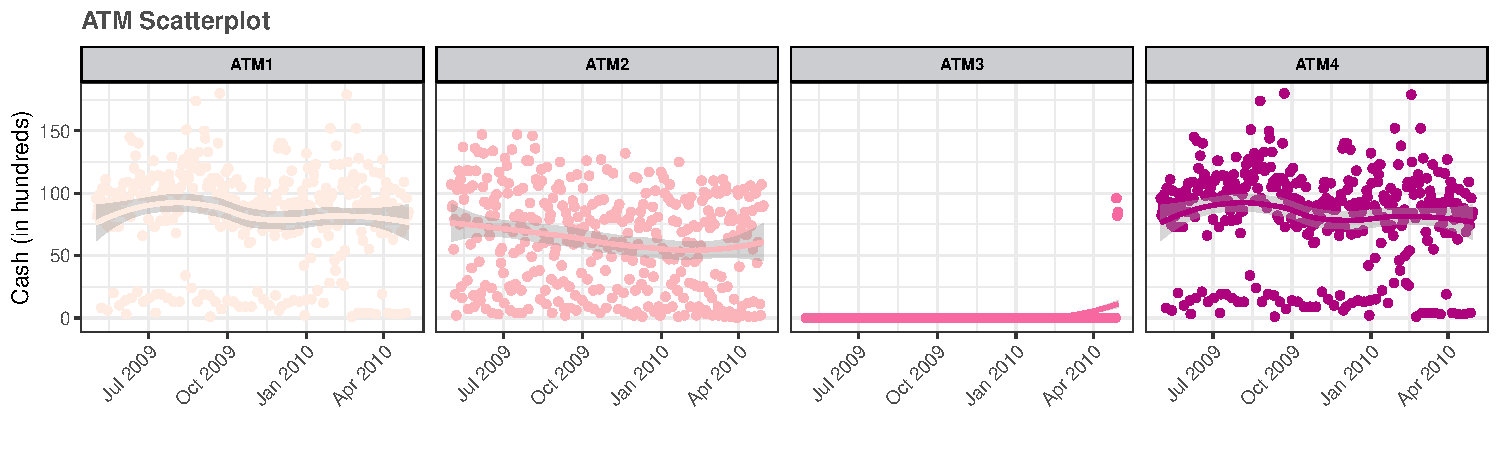
\includegraphics{Part-A-JM_files/figure-latex/unnamed-chunk-2-1.pdf}

\hypertarget{timeseries-plots}{%
\section{Timeseries Plots}\label{timeseries-plots}}

The time series plots show high weekly variance as suspected in from our
scatterplots. We can see again that time series for ATM3 only contains 3
transactions, thus we deemed this series not suitable for modeling and
forecasting. As a result, our following sections will not include
extrapolation on this series.

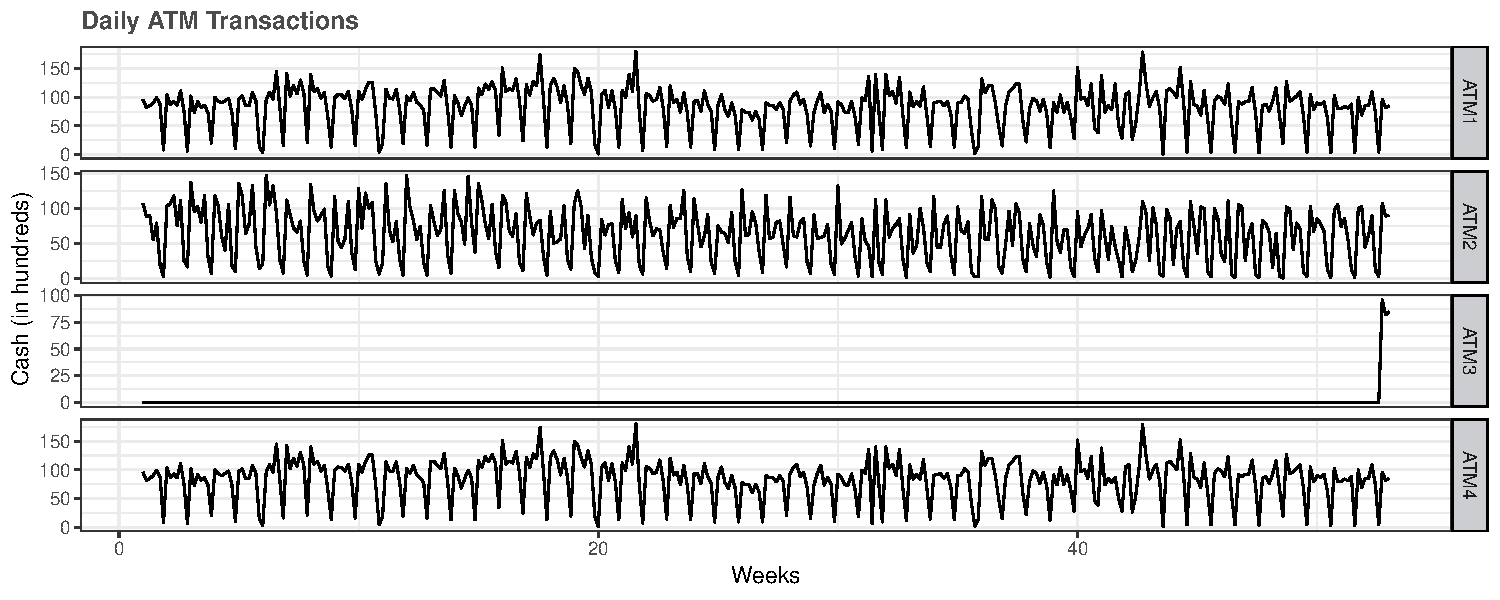
\includegraphics{Part-A-JM_files/figure-latex/unnamed-chunk-3-1.pdf}

\hypertarget{evaluation}{%
\section{Evaluation}\label{evaluation}}

We constructed our initial timeseries using a weekly frequency. Our ACF
plots for each ATM showcases large, decreasing lags starting at 7. This
pattern continues in a multiple of seven, which confirms our assumption
about seasonality within the observed data. These lags are indicative of
a weekly pattern.

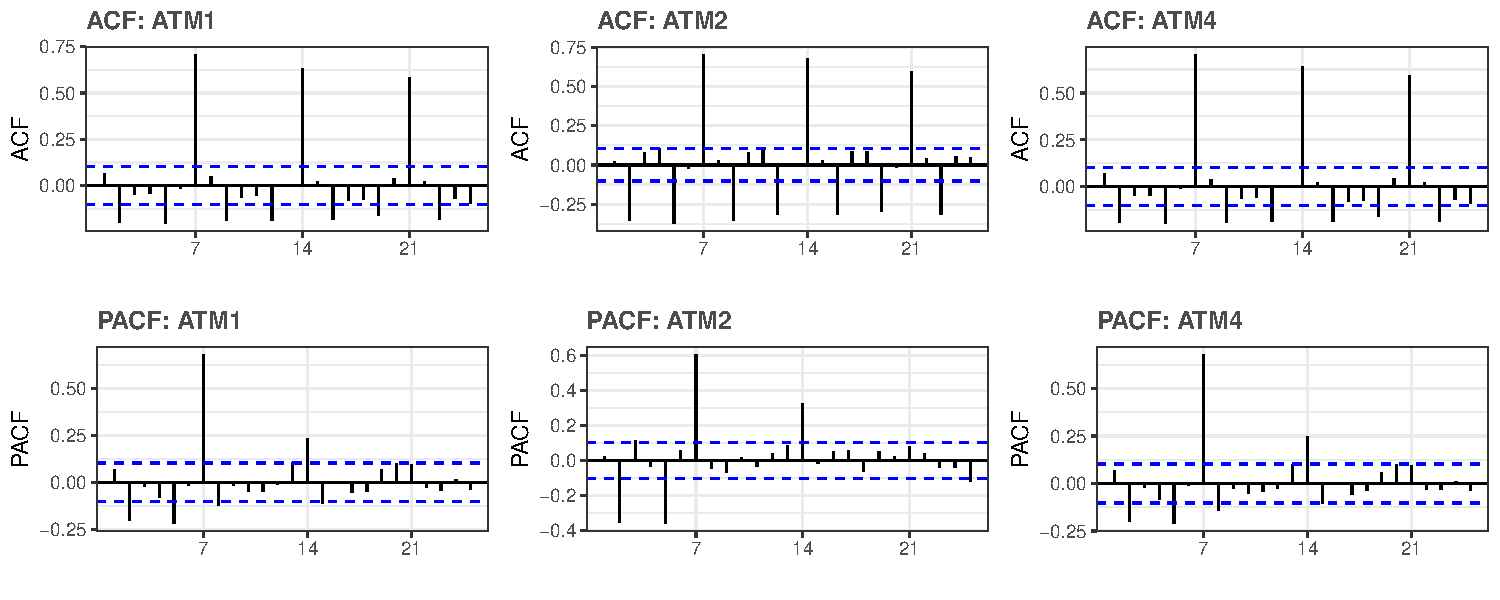
\includegraphics{Part-A-JM_files/figure-latex/unnamed-chunk-4-1.pdf}

Our plots further suggest that the ATM data is non-stationary. We
performed a unit root test using the \texttt{ur.kpss()} function to
confirm this observation. The test results below show that differencing
is required on all ATM2 and ATM4 series. ATM1 falls just below the
cut-off critical value, but could still use differencing due to the
observed seasonal pattern.

\begin{table}[H]

\caption{\label{tab:unnamed-chunk-5}KPSS unit root test}
\centering
\begin{tabular}{l|l|l}
\hline
\textbf{ATM} & \textbf{No-Diff} & \textbf{Diff-1}\\
\hline
\rowcolor{gray!6}  ATM1 & 0.4967 & 0.0219\\
\hline
ATM2 & 2.0006 & 0.016\\
\hline
\rowcolor{gray!6}  ATM4 & 0.5182 & 0.0211\\
\hline
\end{tabular}
\end{table}

\hypertarget{modeling}{%
\subsection{Modeling}\label{modeling}}

We used \texttt{auto.arima()} and set \texttt{D=1} to account for
seasonal differencing of our data to select the best ARIMA models. The
full models and accuracy statistics for each series can be viewed in the
appendix.

\begin{itemize}
\tightlist
\item
  \textbf{ATM1}: ARIMA\((0,0,2)(0,1,1)_7\)
\item
  \textbf{ATM2}: ARIMA\((2,0,2)(0,1,1)_7\)
\item
  \textbf{ATM4}: ARIMA\((0,0,2)(0,1,1)_7\)
\end{itemize}

The following ACF plots show us that our differentiated data is now
stationary. Further, the residual histograms follow a relatively normal
distribution, which confirms that the models adequately fits the
observed data.

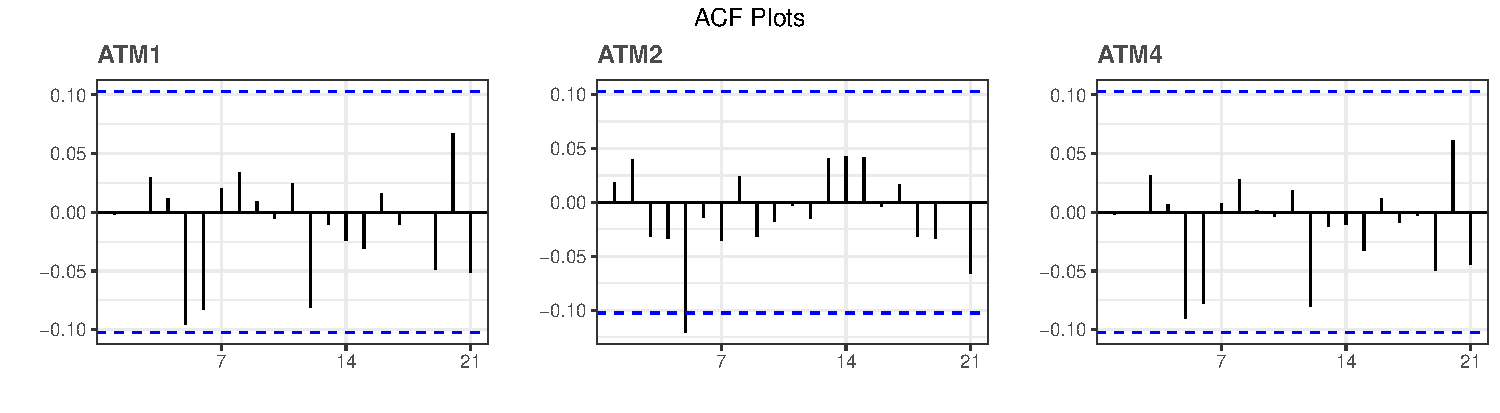
\includegraphics{Part-A-JM_files/figure-latex/unnamed-chunk-6-1.pdf}
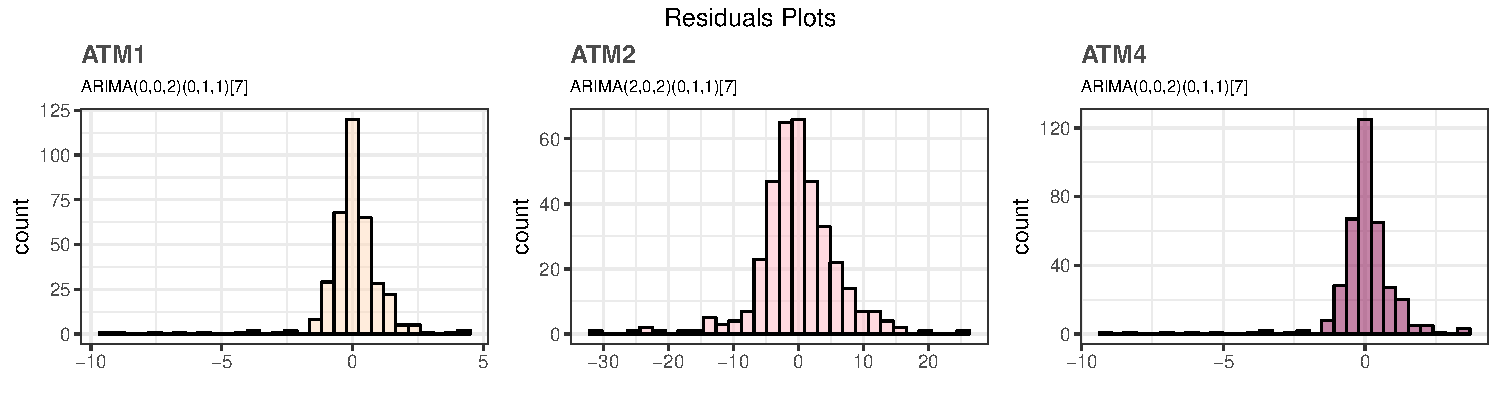
\includegraphics{Part-A-JM_files/figure-latex/unnamed-chunk-6-2.pdf}

\hypertarget{forecast}{%
\section{Forecast}\label{forecast}}

Finally, we applied a forecast to each series for 31 days to predict
cash withdrawals in May 2010. The forecast spans across 5 weeks and
follows similiar trend and seasonality to the fitted data. The numeric
forecasts can be viewed in a table output in the appendix section and
are also located within our data output folder.

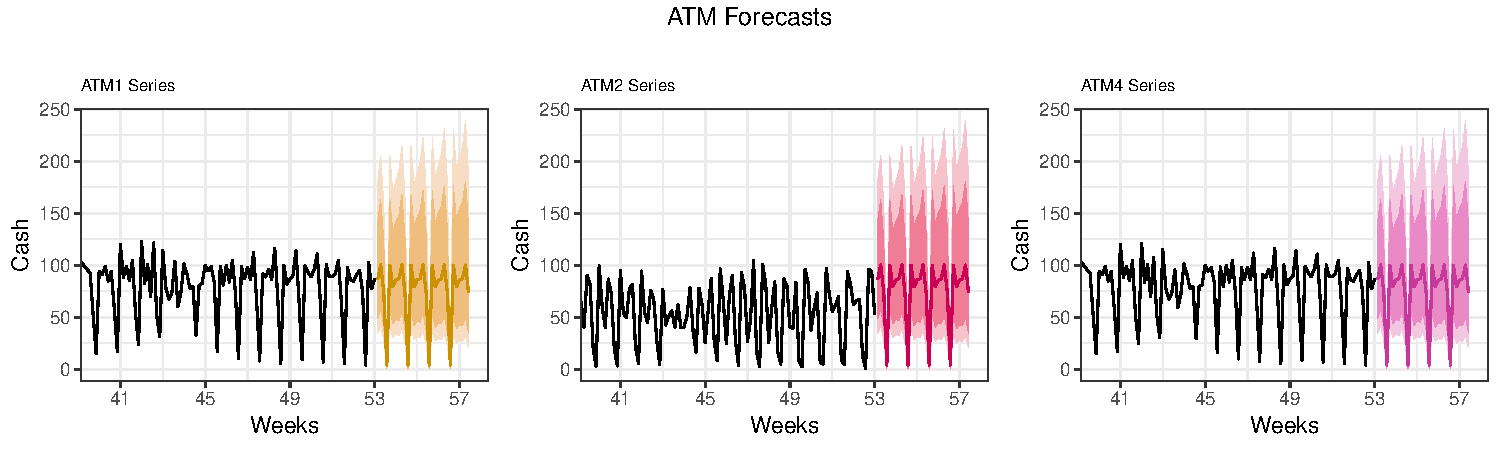
\includegraphics{Part-A-JM_files/figure-latex/unnamed-chunk-7-1.pdf}

\hypertarget{Appendix}{%
\chapter*{Appendix}\label{Appendix}}
\addcontentsline{toc}{chapter}{Appendix}

\hypertarget{Part-A}{%
\section*{Part A}\label{Part-A}}
\addcontentsline{toc}{section}{Part A}

\hypertarget{Part-A-arima}{%
\subsection*{ARIMA Model Summary}\label{Part-A-arima}}
\addcontentsline{toc}{subsection}{ARIMA Model Summary}

\textbf{\texttt{ATM1}:}

\begin{verbatim}
FALSE Series: ATM1_ts 
FALSE ARIMA(0,0,2)(0,1,1)[7] 
FALSE Box Cox transformation: lambda= 0.2584338 
FALSE 
FALSE Coefficients:
FALSE          ma1      ma2     sma1
FALSE       0.1085  -0.1089  -0.6425
FALSE s.e.  0.0524   0.0521   0.0431
FALSE 
FALSE sigma^2 estimated as 1.726:  log likelihood=-606.1
FALSE AIC=1220.2   AICc=1220.32   BIC=1235.72
\end{verbatim}

\textbf{\texttt{ATM2}:}

\begin{verbatim}
FALSE Series: ATM2_ts 
FALSE ARIMA(2,0,2)(0,1,1)[7] 
FALSE Box Cox transformation: lambda= 0.661752 
FALSE 
FALSE Coefficients:
FALSE           ar1      ar2     ma1     ma2     sma1
FALSE       -0.4238  -0.8978  0.4766  0.7875  -0.7064
FALSE s.e.   0.0592   0.0473  0.0883  0.0608   0.0417
FALSE 
FALSE sigma^2 estimated as 38.94:  log likelihood=-1162.96
FALSE AIC=2337.93   AICc=2338.17   BIC=2361.21
\end{verbatim}

\textbf{\texttt{ATM4}:}

\begin{verbatim}
FALSE Series: ATM4_ts 
FALSE ARIMA(0,0,2)(0,1,1)[7] 
FALSE Box Cox transformation: lambda= 0.2328582 
FALSE 
FALSE Coefficients:
FALSE          ma1      ma2     sma1
FALSE       0.1095  -0.1088  -0.6474
FALSE s.e.  0.0524   0.0523   0.0420
FALSE 
FALSE sigma^2 estimated as 1.439:  log likelihood=-573.5
FALSE AIC=1154.99   AICc=1155.11   BIC=1170.52
\end{verbatim}

\hypertarget{Part-A-FC}{%
\subsection*{Point Forecasts}\label{Part-A-FC}}
\addcontentsline{toc}{subsection}{Point Forecasts}

\begin{table}[H]

\caption{\label{tab:unnamed-chunk-11}ATM Mean Point Forecast}
\centering
\begin{tabular}{l|l|l|l|l}
\hline
\textbf{Date} & \textbf{ATM1} & \textbf{ATM2} & \textbf{ATM3} & \textbf{ATM4}\\
\hline
\rowcolor{gray!6}  2010-05-01 & 86.6822230334281 & 65.9130078295388 & NA & 86.7148793513953\\
\hline
2010-05-02 & 100.569237833094 & 71.2678744758685 & NA & 100.581688969852\\
\hline
\rowcolor{gray!6}  2010-05-03 & 73.710292000956 & 11.4694658108709 & NA & 73.645362194735\\
\hline
2010-05-04 & 4.22902938718943 & 2.46415237936744 & NA & 4.22143290375228\\
\hline
\rowcolor{gray!6}  2010-05-05 & 100.159253208527 & 98.3397063045857 & NA & 100.159422079885\\
\hline
2010-05-06 & 79.3467329167084 & 89.0607216505235 & NA & 79.3417211032809\\
\hline
\rowcolor{gray!6}  2010-05-07 & 85.7390398914344 & 66.0684601266365 & NA & 85.7781984478913\\
\hline
2010-05-08 & 87.1797624007239 & 65.9067170158147 & NA & 87.218337497544\\
\hline
\rowcolor{gray!6}  2010-05-09 & 100.388112929695 & 71.3008782172556 & NA & 100.395109536387\\
\hline
2010-05-10 & 73.710292000956 & 11.4650527078295 & NA & 73.645362194735\\
\hline
\rowcolor{gray!6}  2010-05-11 & 4.22902938718943 & 2.45577466621943 & NA & 4.22143290375228\\
\hline
2010-05-12 & 100.159253208527 & 98.3602657501897 & NA & 100.159422079885\\
\hline
\rowcolor{gray!6}  2010-05-13 & 79.3467329167084 & 89.0776223553505 & NA & 79.3417211032809\\
\hline
2010-05-14 & 85.7390398914344 & 66.0458523021009 & NA & 85.7781984478913\\
\hline
\rowcolor{gray!6}  2010-05-15 & 87.1797624007239 & 65.9025868757576 & NA & 87.218337497544\\
\hline
2010-05-16 & 100.388112929695 & 71.3235063276986 & NA & 100.395109536387\\
\hline
\rowcolor{gray!6}  2010-05-17 & 73.710292000956 & 11.4619371370152 & NA & 73.645362194735\\
\hline
2010-05-18 & 4.22902938718943 & 2.45005983249313 & NA & 4.22143290375228\\
\hline
\rowcolor{gray!6}  2010-05-19 & 100.159253208527 & 98.3744953596224 & NA & 100.159422079885\\
\hline
2010-05-20 & 79.3467329167084 & 89.0890848253535 & NA & 79.3417211032809\\
\hline
\rowcolor{gray!6}  2010-05-21 & 85.7390398914344 & 66.0302973545638 & NA & 85.7781984478913\\
\hline
2010-05-22 & 87.1797624007239 & 65.8998808213307 & NA & 87.218337497544\\
\hline
\rowcolor{gray!6}  2010-05-23 & 100.388112929695 & 71.3390190248587 & NA & 100.395109536387\\
\hline
2010-05-24 & 73.710292000956 & 11.4597394828691 & NA & 73.645362194735\\
\hline
\rowcolor{gray!6}  2010-05-25 & 4.22902938718943 & 2.44616060460193 & NA & 4.22143290375228\\
\hline
2010-05-26 & 100.159253208527 & 98.3843423320737 & NA & 100.159422079885\\
\hline
\rowcolor{gray!6}  2010-05-27 & 79.3467329167084 & 89.0968573387821 & NA & 79.3417211032809\\
\hline
2010-05-28 & 85.7390398914344 & 66.0195955091203 & NA & 85.7781984478913\\
\hline
\rowcolor{gray!6}  2010-05-29 & 87.1797624007239 & 65.8981117895746 & NA & 87.218337497544\\
\hline
2010-05-30 & 100.388112929695 & 71.3496527614802 & NA & 100.395109536387\\
\hline
\rowcolor{gray!6}  2010-05-31 & 73.710292000956 & 11.4581905724258 & NA & 73.645362194735\\
\hline
\end{tabular}
\end{table}

\newpage

\hypertarget{Part-A-RScript}{%
\subsection*{R Script}\label{Part-A-RScript}}
\addcontentsline{toc}{subsection}{R Script}

\begin{Shaded}
\begin{Highlighting}[]
\CommentTok{# load data}
\NormalTok{atm_data <-}\StringTok{ }\KeywordTok{read_excel}\NormalTok{(}\StringTok{"data/ATM624Data.xlsx"}\NormalTok{) }

\CommentTok{# clean dataframe}
\NormalTok{atm <-}\StringTok{ }\NormalTok{atm_data }\OperatorTok\StringTok{ }
\StringTok{  }\CommentTok{# create wide dataframe}
\StringTok{  }\KeywordTok{spread}\NormalTok{(ATM, Cash) }\OperatorTok\StringTok{ }
\StringTok{  }\CommentTok{# remove NA column using function from janitor package}
\StringTok{  }\KeywordTok{remove_empty}\NormalTok{(}\DataTypeTok{which =} \StringTok{"cols"}\NormalTok{) }\OperatorTok
\StringTok{  }\CommentTok{# filter unobserved values from May 2010}
\StringTok{  }\KeywordTok{filter}\NormalTok{(DATE }\OperatorTok{<}\StringTok{ }\KeywordTok{as.Date}\NormalTok{(}\StringTok{"2010-05-01"}\NormalTok{)) }\OperatorTok
\StringTok{  }\CommentTok{# ensure dates are ascending}
\StringTok{  }\KeywordTok{arrange}\NormalTok{(DATE) }

\NormalTok{atm}\OperatorTok{$}\NormalTok{ATM2[}\KeywordTok{is.na}\NormalTok{(atm}\OperatorTok{$}\NormalTok{ATM2)] <-}\StringTok{ }\KeywordTok{mean}\NormalTok{(atm}\OperatorTok{$}\NormalTok{ATM2, }\DataTypeTok{na.rm =} \OtherTok{TRUE}\NormalTok{) }\CommentTok{## remove NA}
\NormalTok{atm}\OperatorTok{$}\NormalTok{ATM4[}\KeywordTok{which.max}\NormalTok{(atm}\OperatorTok{$}\NormalTok{ATM4)] <-}\StringTok{ }\KeywordTok{mean}\NormalTok{(atm}\OperatorTok{$}\NormalTok{ATM4, }\DataTypeTok{na.rm =} \OtherTok{TRUE}\NormalTok{) }\CommentTok{## remove outlier}

\CommentTok{# create TS with weekly frequency & subset data}
\NormalTok{atm_ts <-}\StringTok{ }\NormalTok{atm }\OperatorTok\StringTok{ }\KeywordTok{select}\NormalTok{(}\OperatorTok{-}\NormalTok{DATE) }\OperatorTok\StringTok{ }\KeywordTok{ts}\NormalTok{(}\DataTypeTok{start=}\DecValTok{1}\NormalTok{,  }\DataTypeTok{frequency =} \DecValTok{7}\NormalTok{)}
\NormalTok{ATM1_ts <-}\StringTok{ }\NormalTok{atm_ts[,}\DecValTok{1}\NormalTok{]; ATM2_ts <-}\StringTok{ }\NormalTok{atm_ts[,}\DecValTok{2}\NormalTok{]; ATM4_ts <-}\StringTok{ }\NormalTok{atm_ts[,}\DecValTok{4}\NormalTok{]}

\CommentTok{#unit root test}
\CommentTok{## no diff}
\NormalTok{ATM1_ur <-}\KeywordTok{ur.kpss}\NormalTok{(ATM1_ts)}
\NormalTok{ATM2_ur <-}\KeywordTok{ur.kpss}\NormalTok{(ATM2_ts)}
\NormalTok{ATM4_ur <-}\KeywordTok{ur.kpss}\NormalTok{(ATM4_ts)}
\CommentTok{## first order diff}
\NormalTok{ATM1d_ur <-}\KeywordTok{ur.kpss}\NormalTok{(}\KeywordTok{diff}\NormalTok{(ATM1_ts, }\DataTypeTok{lag=}\DecValTok{7}\NormalTok{))}
\NormalTok{ATM2d_ur <-}\KeywordTok{ur.kpss}\NormalTok{(}\KeywordTok{diff}\NormalTok{(ATM2_ts, }\DataTypeTok{lag=}\DecValTok{7}\NormalTok{))}
\NormalTok{ATM4d_ur <-}\KeywordTok{ur.kpss}\NormalTok{(}\KeywordTok{diff}\NormalTok{(ATM4_ts, }\DataTypeTok{lag=}\DecValTok{7}\NormalTok{))}

\CommentTok{# AUTO.ARIMA function; set D=1 for seasonal differencing}
\NormalTok{ATM1_AA <-}\KeywordTok{auto.arima}\NormalTok{(ATM1_ts, }\DataTypeTok{D =} \DecValTok{1}\NormalTok{, }\DataTypeTok{lambda =} \StringTok{"auto"}\NormalTok{, }\DataTypeTok{approximation =}\NormalTok{ F, }\DataTypeTok{stepwise =}\NormalTok{ T)}
\NormalTok{ATM2_AA <-}\KeywordTok{auto.arima}\NormalTok{(ATM2_ts, }\DataTypeTok{D =} \DecValTok{1}\NormalTok{, }\DataTypeTok{lambda =} \StringTok{"auto"}\NormalTok{, }\DataTypeTok{approximation =}\NormalTok{ F, }\DataTypeTok{stepwise =}\NormalTok{ T)}
\NormalTok{ATM4_AA <-}\KeywordTok{auto.arima}\NormalTok{(ATM4_ts, }\DataTypeTok{D =} \DecValTok{1}\NormalTok{, }\DataTypeTok{lambda =} \StringTok{"auto"}\NormalTok{, }\DataTypeTok{approximation =}\NormalTok{ F, }\DataTypeTok{stepwise =}\NormalTok{ T)}

\CommentTok{# Forecast Results}
\NormalTok{ATM1_fc <-}\StringTok{ }\KeywordTok{forecast}\NormalTok{(ATM1_AA,}\DataTypeTok{h=}\DecValTok{31}\NormalTok{)}
\NormalTok{ATM2_fc <-}\StringTok{ }\KeywordTok{forecast}\NormalTok{(ATM2_AA,}\DataTypeTok{h=}\DecValTok{31}\NormalTok{)}
\NormalTok{ATM4_fc <-}\StringTok{ }\KeywordTok{forecast}\NormalTok{(ATM4_AA,}\DataTypeTok{h=}\DecValTok{31}\NormalTok{)}

\CommentTok{# Revert results back into original form}
\NormalTok{date <-}\StringTok{ }\KeywordTok{as.character}\NormalTok{(}\KeywordTok{seq}\NormalTok{(}\KeywordTok{as.Date}\NormalTok{(}\StringTok{'2010-05-01'}\NormalTok{), }\DataTypeTok{length.out=}\DecValTok{31}\NormalTok{, }\DataTypeTok{by=}\DecValTok{1}\NormalTok{))}
\NormalTok{ATM_FC <-}\StringTok{  }\KeywordTok{cbind}\NormalTok{(}\StringTok{"Date"}\NormalTok{=date, }\StringTok{"ATM1"}\NormalTok{=ATM1_fc}\OperatorTok{$}\NormalTok{mean, }\StringTok{"ATM2"}\NormalTok{=ATM2_fc}\OperatorTok{$}\NormalTok{mean,}
                 \StringTok{"ATM3"}\NormalTok{=}\KeywordTok{c}\NormalTok{(}\OtherTok{NA}\NormalTok{,}\OtherTok{NA}\NormalTok{,}\OtherTok{NA}\NormalTok{,}\OtherTok{NA}\NormalTok{),}\StringTok{"ATM4"}\NormalTok{=ATM4_fc}\OperatorTok{$}\NormalTok{mean) }\OperatorTok\StringTok{ }\KeywordTok{as.data.frame}\NormalTok{()}

\CommentTok{# Save output}
\KeywordTok{write.csv}\NormalTok{(ATM_FC, }\DataTypeTok{file=}\StringTok{"forecasts/ATM_ARIMA_FC.csv"}\NormalTok{)}
\end{Highlighting}
\end{Shaded}


\end{document}
